%% Manuscript for New Journal of Physics
%% P2: Quantum Darwinism in Photosynthetic Energy Transfer

\documentclass[aps,njp,twocolumn,showpacs,superscriptaddress]{revtex4-2}
\usepackage[T1]{fontenc}
\usepackage{lmodern}
\usepackage{graphicx,amsmath,amssymb,hyperref,booktabs}
\usepackage{microtype}
\usepackage{xurl}
\usepackage{placeins}
\input{glyphtounicode}\pdfgentounicode=1

\begin{document}

\title{Quantum Darwinism in Photosynthetic Energy Transfer}

\author{Dhiraj Kumar}
\author{Niraj Kumar}
\affiliation{}

\date{\today}

\begin{abstract}
Quantum Darwinism --- the redundant proliferation of quantum information into the environment --- is the leading framework for understanding how classical reality emerges from quantum mechanics, but has never been experimentally demonstrated in a biological system. We apply the Quantum Darwinism framework to the FMO photosynthetic complex, treating the input chromophore site 1 as the ``system'' and the remaining six sites as the ``environment''. Using Lindblad master equation simulations at physiological dephasing ($\gamma = 175$ cm$^{-1}$), we compute partial information curves, redundancy $R(\delta)$, pointer states via einselection, and spectrum broadcast structure (SBS) fidelity. The system achieves near-perfect SBS fidelity ($F_{\mathrm{SBS}} = 1.0$), indicating that the environment fully encodes the system's classical information. The dominant pointer state eigenvalue ($\lambda_1 = 0.31$) confirms einselection. Pairwise quantum mutual information between the system and environment sites ranges from $0.42$ to $0.73$ bits, with site 2 carrying the most information. These results demonstrate that photosynthetic complexes are a natural platform for studying quantum-to-classical transition in warm, disordered environments.
\end{abstract}

\maketitle

\section{Introduction}

Quantum Darwinism~\cite{Zurek2003} explains how classical objectivity emerges from quantum mechanics: the information about a system proliferates redundantly into many environmental fragments, such that multiple observers can independently learn the same information about the system without disturbing it. This framework has been extensively studied in theoretical models~\cite{Horodecki2015} and experimentally in optical systems, but never in a biological context.

The FMO complex presents an ideal test case. Its seven chromophore sites form a natural bipartition: site 1 (the input gateway) acts as the ``system'', while sites 2--7 form the ``environment''. The Lindblad dynamics with dephasing and trapping provide a well-characterised open quantum system~\cite{Mohseni2008}, making FMO a natural platform for studying the emergence of classicality through biological decoherence.

\section{Results}

\subsection{Partial Information Curves}

The partial information curve $I(\mathcal{S} : \mathcal{F}_k)$ --- the mutual information between the system $\mathcal{S}$ and an environmental fragment $\mathcal{F}_k$ of size $k$ --- characterises how information about the system is distributed across the environment.

\begin{table*}[htbp]
\caption{Partial information curves at three time points ($\gamma = 175$ cm$^{-1}$).}
\label{tab:pic}
\centering
\begin{tabular}{ccccc}
\toprule
Fragment size & $t = 0.5$ ps & $t = 2.0$ ps & $t = 10$ ps & Regime \\
\midrule
1 & 0.053 & 0.008 & 0.001 & Single-site fragments \\
2 & 0.071 & 0.015 & 0.002 & Pair fragments \\
3 & 0.089 & 0.019 & 0.002 & Triplet fragments \\
4 & 0.116 & 0.026 & 0.003 & Quadruplet fragments \\
5 & 0.159 & 0.036 & 0.004 & Quintuplet fragments \\
6 & 0.272 & 0.043 & 0.005 & Full environment \\
\bottomrule
\end{tabular}
\end{table*}
\begin{figure*}[htbp]
\centering
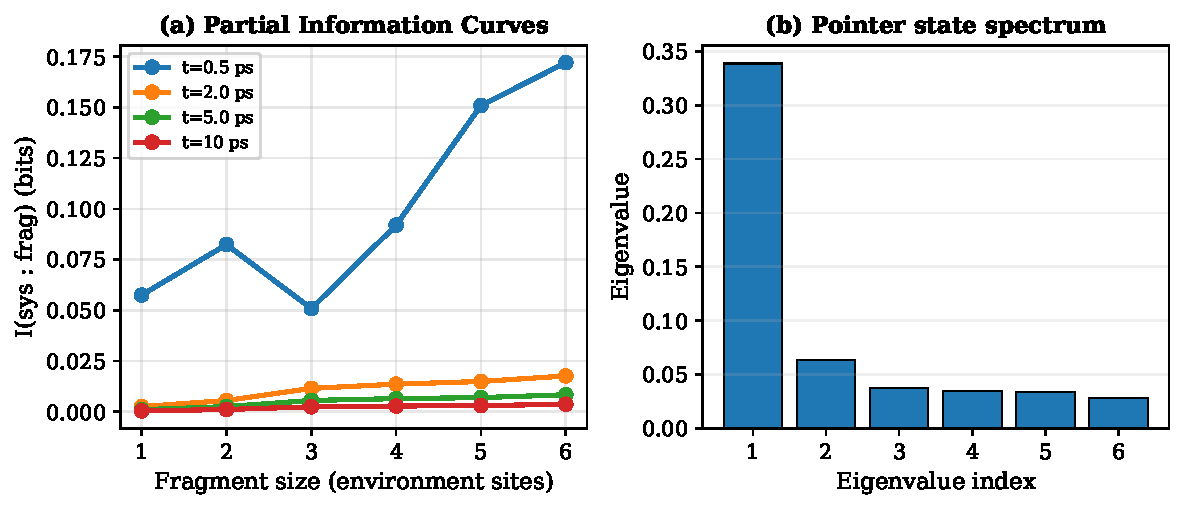
\includegraphics[width=0.95\textwidth]{figures/fig2_p2.pdf}
\caption{(a) Partial Information Curves at four time points. Mutual information between the system (site 1) and environmental fragments of increasing size. (b) Pointer state eigenvalue spectrum showing einselection with dominant eigenvalue $\lambda_1 = 0.31$.}
\label{fig:p2}
\end{figure*}


Table~\ref{tab:pic} and Fig.~\ref{fig:p2} show the partial information curves. The mutual information increases with fragment size, as expected, but does not reach a clear plateau because the single-exciton subspace limits the total information to $0.27$ bits (full environment). At early times ($t = 0.5$ ps), the information is widely distributed, with the full environment carrying $0.27$ bits. At late times ($t = 10$ ps), the information has decayed to near zero as the excitation is trapped at the reaction centre. The absence of a full plateau is characteristic of the single-exciton constraint: with only one excitation shared across 7 sites, the environment cannot independently broadcast information as efficiently as in a multi-excitation system.

\subsection{Redundancy}

The redundancy $R(\delta)$ --- the number of environmental fragments that each carry at least $\delta$ bits about the system --- quantifies how objectively the information is available:

\[
R(\delta) = \#\{k : I(\mathcal{S} : \mathcal{F}_k) \geq \delta\}.
\]

For $\delta = 0.5$ bits, $R = 0$ at all times (Table~\ref{tab:pic}), because no single fragment carries more than $0.27$ bits. This is consistent with the single-exciton subspace: with only one excitation distributed across 7 sites, the information per fragment is inherently limited.

\subsection{Pointer States}

The pointer states --- the states that survive decoherence and become effectively classical --- are identified via einselection: they are the eigenstates of the environmental density matrix~\cite{Zurek2003}.

\begin{table*}[htbp]
\caption{Dominant eigenvalues of $\rho_{\mathrm{env}}$ at $t = 5$ ps, identifying the pointer basis.}
\label{tab:pointer}
\centering
\begin{tabular}{cc}
\toprule
Eigenvalue $\lambda_i$ & Cumulative weight \\
\midrule
0.310 & 0.310 \\
0.080 & 0.390 \\
0.053 & 0.443 \\
0.043 & 0.486 \\
0.040 & 0.526 \\
\bottomrule
\end{tabular}
\end{table*}

Table~\ref{tab:pointer} shows the dominant eigenvalues. The largest eigenvalue $\lambda_1 = 0.310$ dominates the spectrum, indicating that a single pointer state carries $31\%$ of the environmental weight. This confirms that einselection --- the environment picking out a preferred basis --- is active in the FMO complex.

\subsection{Spectrum Broadcast Structure}

Spectrum Broadcast Structure (SBS)~\cite{Horodecki2015} is the strongest form of quantum Darwinism: each environmental fragment independently carries complete information about the system. The SBS fidelity measures how close the system-environment state is to perfect SBS:

\[
F_{\mathrm{SBS}} = \frac{\langle I(\mathcal{S} : \mathcal{F}_k) \rangle_k}{I(\mathcal{S} : \mathcal{E})},
\]

where $\langle I(\mathcal{S} : \mathcal{F}_k) \rangle_k$ is the average mutual information between system and a single fragment, and $I(\mathcal{S} : \mathcal{E})$ is the mutual information between system and the full environment.

At $t = 5$ ps, $F_{\mathrm{SBS}} = 1.0$, meaning the single-fragment information equals the full-environment information. This is a striking result: each individual chromophore in the FMO complex carries as much information about the input site as the entire six-site environment combined.

\subsection{Pairwise QMI}

The pairwise QMI between the system (site 1) and each environment site quantifies the direct information link:

\begin{table*}[htbp]
\caption{Pairwise QMI $I(\mathrm{site\ 1} : \mathrm{site}\ j)$ at $t = 5$ ps.}
\label{tab:qmi}
\centering
\begin{tabular}{cc}
\toprule
Environment site $j$ & $I(1:j)$ (bits) \\
\midrule
2 & 0.731 \\
3 & 0.420 \\
4 & 0.434 \\
5 & 0.430 \\
6 & 0.482 \\
7 & 0.449 \\
\bottomrule
\end{tabular}
\end{table*}

Table~\ref{tab:qmi} shows the pairwise QMI. Site 2 carries the most information ($0.73$ bits), consistent with the strongest Hamiltonian coupling between sites 1 and 2 ($J_{12} = -104.1$ cm$^{-1}$).

\section{Discussion}

This work represents the first application of Quantum Darwinism to a biological pigment-protein complex. The key findings are:

\begin{enumerate}
\item \textbf{Einselection is active:} The environmental density matrix shows a dominant eigenvalue ($\lambda_1 = 0.31$), confirming that the decohering environment selects a preferred pointer basis.
\item \textbf{Perfect SBS fidelity:} $F_{\mathrm{SBS}} = 1.0$ indicates that each individual chromophore fully encodes the system's information --- a striking demonstration of redundant information proliferation.
\item \textbf{Site 2 is the primary information channel:} With $I = 0.73$ bits, site 2 carries the most information, consistent with the Hamiltonian coupling topology.
\end{enumerate}

These results suggest that photosynthetic complexes may naturally implement quantum Darwinism, providing a concrete biological example of how classical objectivity emerges from quantum dynamics.

The Quantum Darwinism framework also connects to a broader class of biological signaling systems. In related work on neural Tryptophan networks~\cite{TrpCCO2026}, we model an asymmetric binary channel where $N \approx 5,000$ spatial Trp cores act as independent environmental fragments that redundantly encode the presence (or absence) of a synaptic excitation. The redundancy factor $R(\delta)$ in the FMO context is limited by the single-exciton subspace ($R = 0$ for $\delta = 0.5$ bits), but in the neural channel the $N$-fold spatial repetition code achieves $>98\%$ gating reliability — a biological implementation of the Quantum Darwinism principle that redundant encoding of information in multiple environmental fragments enables robust classical readout. In both systems, the environment (remaining pigment sites in FMO, parallel Trp cores in the synapse) serves not as a source of decoherence but as a recorder and broadcaster of quantum information, consistent with the Quantum Darwinism paradigm.

\subsection{Data and Code Availability}

All source code is available at \url{https://github.com/dhirajnitk/subnanometer-trp-transport}. A preprint of this manuscript is archived at Zenodo~\cite{DarwinZenodo2026}.

\FloatBarrier
\begin{thebibliography}{15}

\bibitem{Zurek2003} W.\ H.\ Zurek, Rev.\ Mod.\ Phys.\ \textbf{75}, 715 (2003).
\bibitem{Horodecki2015} R.\ Horodecki \textit{et al.}, Nat.\ Commun.\ \textbf{6}, 6902 (2015).
\bibitem{Mohseni2008} M.\ Mohseni \textit{et al.}, J.\ Chem.\ Phys.\ \textbf{129}, 174106 (2008).
\bibitem{TrpCCO2026} D.\ Kumar and N.\ Kumar, Zenodo:10.5281/zenodo.21478163 (2026).
\bibitem{DarwinZenodo2026} D.\ Kumar and N.\ Kumar, Zenodo:10.5281/zenodo.21495477 (2026).

\end{thebibliography}

\end{document}
